\documentclass{standalone}
\usepackage{pgfplots}
\pgfplotsset{compat=1.17}

\definecolor{tab_blue}{HTML}{1F77B4}
\definecolor{tab_orange}{HTML}{FF7F0E}
\definecolor{tab_green}{HTML}{2CA02C}
\definecolor{tab_red}{HTML}{D62728}

\begin{document}
    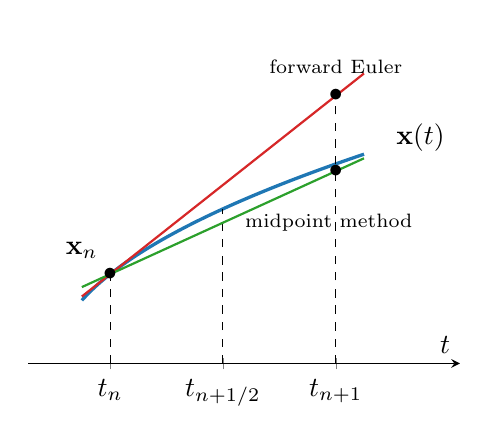
\begin{tikzpicture}[baseline]
        \begin{axis}[
            scale=0.8, % scale
            % view = {0}{90},
            xmin=-0.18,xmax=2.88,ymin=-0.08,ymax=2.38, % range of plot
            % legend style={at={(axis cs: 1,0)}, anchor=south east}, % position of legends
            % unit vector ratio = {1, 1, 1}, % aspect ratio
            unit vector ratio = {1, 1}, % aspect ratio
            axis lines = middle, % middle or box
            %axis x line = bottom, % top, middle, bottom, none: axis x line* = ... removes arrow heads
            %axis y line = left, % left, center, right, none: axis y line* = ... removes arrow heads
            xlabel = {$t$}, % axis labels 
            y axis line style = {draw=none},
            xtick = {0.4, 1.2, 2.0},
            xticklabels = {$t_n$, $t_{n+1/2}$, $t_{n+1}$},
            ytick = {-1},
        ]
            % \addplot3[blue, quiver={u={y}, v={-x}}, domain=-1.5:1.5, y domain=-1.5:1.5, samples=12, -latex] (x, y, 0);
            \addplot[color=tab_blue, domain=0.2:2.2, samples=100, very thick] {sqrt(x)};
            \addplot[domain=0:0.4, dashed] ({0.4}, {sqrt(x)}); 
            \addplot[domain=0:1.2, dashed] ({1.2}, {sqrt(x)}); 
            \addplot[domain=-0.4:2.0, dashed] ({2.0}, {x/(2*sqrt(0.4)) + sqrt(0.4)/2}); 
            \addplot[color=tab_red, domain=0.2:2.2, thick] {x/(2*sqrt(0.4)) + sqrt(0.4)/2};
            % \addplot[color=tab_green, domain=0.5:2.1, thick] {x/(2*sqrt(1.2)) + sqrt(1.2)/2};
            \addplot[color=tab_green, domain=0.2:2.2, thick] {x/(2*sqrt(1.2)) - 0.4/(2*sqrt(1.2)) + sqrt(0.4)};
            \node at (0.4, {sqrt(0.4)}) {$\bullet$};
            \node at (0.2, 0.8) {$\mathbf{x}_n$};
            \node at (2.0, {2.0/(2*sqrt(0.4)) + sqrt(0.4)/2}) {$\bullet$};
            \node at (2.6, 1.6) {$\mathbf{x}(t)$};
            \node at (2.0, 2.1) {\scriptsize forward Euler};
            \node at (2.0, {2.0/(2*sqrt(1.2)) - 0.4/(2*sqrt(1.2)) + sqrt(0.4)}) {$\bullet$}; 
            \node at (1.95, 1.0) {\scriptsize midpoint method};
        \end{axis}
    \end{tikzpicture}
\end{document}